\documentclass[twoside]{book}

% Packages required by doxygen
\usepackage{fixltx2e}
\usepackage{calc}
\usepackage{doxygen}
\usepackage[export]{adjustbox} % also loads graphicx
\usepackage{graphicx}
\usepackage[utf8]{inputenc}
\usepackage{makeidx}
\usepackage{multicol}
\usepackage{multirow}
\PassOptionsToPackage{warn}{textcomp}
\usepackage{textcomp}
\usepackage[nointegrals]{wasysym}
\usepackage[table]{xcolor}

% Font selection
\usepackage[T1]{fontenc}
\usepackage[scaled=.90]{helvet}
\usepackage{courier}
\usepackage{amssymb}
\usepackage{sectsty}
\renewcommand{\familydefault}{\sfdefault}
\allsectionsfont{%
  \fontseries{bc}\selectfont%
  \color{darkgray}%
}
\renewcommand{\DoxyLabelFont}{%
  \fontseries{bc}\selectfont%
  \color{darkgray}%
}
\newcommand{\+}{\discretionary{\mbox{\scriptsize$\hookleftarrow$}}{}{}}

% Page & text layout
\usepackage{geometry}
\geometry{%
  a4paper,%
  top=2.5cm,%
  bottom=2.5cm,%
  left=2.5cm,%
  right=2.5cm%
}
\tolerance=750
\hfuzz=15pt
\hbadness=750
\setlength{\emergencystretch}{15pt}
\setlength{\parindent}{0cm}
\setlength{\parskip}{3ex plus 2ex minus 2ex}
\makeatletter
\renewcommand{\paragraph}{%
  \@startsection{paragraph}{4}{0ex}{-1.0ex}{1.0ex}{%
    \normalfont\normalsize\bfseries\SS@parafont%
  }%
}
\renewcommand{\subparagraph}{%
  \@startsection{subparagraph}{5}{0ex}{-1.0ex}{1.0ex}{%
    \normalfont\normalsize\bfseries\SS@subparafont%
  }%
}
\makeatother

% Headers & footers
\usepackage{fancyhdr}
\pagestyle{fancyplain}
\fancyhead[LE]{\fancyplain{}{\bfseries\thepage}}
\fancyhead[CE]{\fancyplain{}{}}
\fancyhead[RE]{\fancyplain{}{\bfseries\leftmark}}
\fancyhead[LO]{\fancyplain{}{\bfseries\rightmark}}
\fancyhead[CO]{\fancyplain{}{}}
\fancyhead[RO]{\fancyplain{}{\bfseries\thepage}}
\fancyfoot[LE]{\fancyplain{}{}}
\fancyfoot[CE]{\fancyplain{}{}}
\fancyfoot[RE]{\fancyplain{}{\bfseries\scriptsize Generated by Doxygen }}
\fancyfoot[LO]{\fancyplain{}{\bfseries\scriptsize Generated by Doxygen }}
\fancyfoot[CO]{\fancyplain{}{}}
\fancyfoot[RO]{\fancyplain{}{}}
\renewcommand{\footrulewidth}{0.4pt}
\renewcommand{\chaptermark}[1]{%
  \markboth{#1}{}%
}
\renewcommand{\sectionmark}[1]{%
  \markright{\thesection\ #1}%
}

% Indices & bibliography
\usepackage{natbib}
\usepackage[titles]{tocloft}
\setcounter{tocdepth}{3}
\setcounter{secnumdepth}{5}
\makeindex

% Hyperlinks (required, but should be loaded last)
\usepackage{ifpdf}
\ifpdf
  \usepackage[pdftex,pagebackref=true]{hyperref}
\else
  \usepackage[ps2pdf,pagebackref=true]{hyperref}
\fi
\hypersetup{%
  colorlinks=true,%
  linkcolor=blue,%
  citecolor=blue,%
  unicode%
}

% Custom commands
\newcommand{\clearemptydoublepage}{%
  \newpage{\pagestyle{empty}\cleardoublepage}%
}

\usepackage{caption}
\captionsetup{labelsep=space,justification=centering,font={bf},singlelinecheck=off,skip=4pt,position=top}

%===== C O N T E N T S =====

\begin{document}

% Titlepage & ToC
\hypersetup{pageanchor=false,
             bookmarksnumbered=true,
             pdfencoding=unicode
            }
\pagenumbering{roman}
\begin{titlepage}
\vspace*{7cm}
\begin{center}%
{\Large My Project }\\
\vspace*{1cm}
{\large Generated by Doxygen 1.8.11}\\
\end{center}
\end{titlepage}
\clearemptydoublepage
\tableofcontents
\clearemptydoublepage
\pagenumbering{arabic}
\hypersetup{pageanchor=true}

%--- Begin generated contents ---
\chapter{Class Index}
\section{Class List}
Here are the classes, structs, unions and interfaces with brief descriptions\+:\begin{DoxyCompactList}
\item\contentsline{section}{\mbox{\hyperlink{class_events}{Events}} }{\pageref{class_events}}{}
\item\contentsline{section}{\mbox{\hyperlink{class_interface}{Interface}} }{\pageref{class_interface}}{}
\item\contentsline{section}{\mbox{\hyperlink{class_i_o}{IO}} \\*A header file for Input/\+Output (\mbox{\hyperlink{class_i_o}{IO}}) class }{\pageref{class_i_o}}{}
\item\contentsline{section}{\mbox{\hyperlink{class_log}{Log}} \\*A header file \mbox{\hyperlink{class_log}{Log}} class }{\pageref{class_log}}{}
\item\contentsline{section}{\mbox{\hyperlink{class_interface_1_1_menu}{Interface\+::\+Menu}} }{\pageref{class_interface_1_1_menu}}{}
\end{DoxyCompactList}

\chapter{File Index}
\section{File List}
Here is a list of all documented files with brief descriptions\+:\begin{DoxyCompactList}
\item\contentsline{section}{{\bfseries events.\+h} }{\pageref{events_8h}}{}
\item\contentsline{section}{\hyperlink{events_8hpp}{events.\+hpp} }{\pageref{events_8hpp}}{}
\item\contentsline{section}{{\bfseries interface.\+h} }{\pageref{interface_8h}}{}
\item\contentsline{section}{\hyperlink{interface_8hpp}{interface.\+hpp} }{\pageref{interface_8hpp}}{}
\item\contentsline{section}{{\bfseries io.\+h} }{\pageref{io_8h}}{}
\item\contentsline{section}{\hyperlink{io_8hpp}{io.\+hpp} }{\pageref{io_8hpp}}{}
\item\contentsline{section}{{\bfseries log.\+h} }{\pageref{log_8h}}{}
\item\contentsline{section}{\hyperlink{log_8hpp}{log.\+hpp} }{\pageref{log_8hpp}}{}
\item\contentsline{section}{\hyperlink{main_8cpp}{main.\+cpp} \\*Driver for project }{\pageref{main_8cpp}}{}
\end{DoxyCompactList}

\chapter{Class Documentation}
\hypertarget{classEvents}{\section{Events Class Reference}
\label{classEvents}\index{Events@{Events}}
}
\subsection*{Static Public Member Functions}
\begin{DoxyCompactItemize}
\item 
static void \hyperlink{classEvents_a2fdb7c40bf64aa2e23d3d92dc7ab4d35}{user\-Mode} ()
\item 
static void \hyperlink{classEvents_a2217e32868e367ec8d432ce9db2b450e}{admin\-Mode} ()
\end{DoxyCompactItemize}


\subsection{Member Function Documentation}
\hypertarget{classEvents_a2217e32868e367ec8d432ce9db2b450e}{\index{Events@{Events}!admin\-Mode@{admin\-Mode}}
\index{admin\-Mode@{admin\-Mode}!Events@{Events}}
\subsubsection[{admin\-Mode}]{\setlength{\rightskip}{0pt plus 5cm}void Events\-::admin\-Mode (
\begin{DoxyParamCaption}
{}
\end{DoxyParamCaption}
)\hspace{0.3cm}{\ttfamily [static]}}}\label{classEvents_a2217e32868e367ec8d432ce9db2b450e}
\begin{DoxyPrecond}{Precondition}
None 
\end{DoxyPrecond}
\begin{DoxyPostcond}{Postcondition}
Start Admin Mode 
\end{DoxyPostcond}
\begin{DoxyReturn}{Returns}
None 
\end{DoxyReturn}
\hypertarget{classEvents_a2fdb7c40bf64aa2e23d3d92dc7ab4d35}{\index{Events@{Events}!user\-Mode@{user\-Mode}}
\index{user\-Mode@{user\-Mode}!Events@{Events}}
\subsubsection[{user\-Mode}]{\setlength{\rightskip}{0pt plus 5cm}void Events\-::user\-Mode (
\begin{DoxyParamCaption}
{}
\end{DoxyParamCaption}
)\hspace{0.3cm}{\ttfamily [static]}}}\label{classEvents_a2fdb7c40bf64aa2e23d3d92dc7ab4d35}
\begin{DoxyPrecond}{Precondition}
None 
\end{DoxyPrecond}
\begin{DoxyPostcond}{Postcondition}
Start User Mode 
\end{DoxyPostcond}
\begin{DoxyReturn}{Returns}
None 
\end{DoxyReturn}


The documentation for this class was generated from the following files\-:\begin{DoxyCompactItemize}
\item 
/home/w751g500/eecs448/team3\-\_\-project1/\-Source/events.\-h\item 
/home/w751g500/eecs448/team3\-\_\-project1/\-Source/\hyperlink{events_8hpp}{events.\-hpp}\end{DoxyCompactItemize}

\hypertarget{classInterface}{}\section{Interface Class Reference}
\label{classInterface}\index{Interface@{Interface}}
\subsection*{Classes}
\begin{DoxyCompactItemize}
\item 
class \hyperlink{classInterface_1_1Menu}{Menu}
\end{DoxyCompactItemize}
\subsection*{Public Member Functions}
\begin{DoxyCompactItemize}
\item 
\hyperlink{classInterface_a4406d74c75bdfe150bf72be1f1cda8b1}{Interface} ()
\item 
\hyperlink{classInterface_a19179888f29f18f1be54a3dfe98f68c0}{$\sim$\+Interface} ()
\item 
std\+::string \hyperlink{classInterface_a73eee93e24c223cd265b5fb0ca1640b8}{get\+Name} ()
\end{DoxyCompactItemize}
\subsection*{Static Public Member Functions}
\begin{DoxyCompactItemize}
\item 
static void \hyperlink{classInterface_af92bb2aeecc6a19095af23fa78b49451}{clear\+Screen} ()
\item 
static void \hyperlink{classInterface_ab235ba2f0184e3fbfd5d5a64d5eb85ef}{Wait} (std\+::string wait\+\_\+string)
\item 
static void \hyperlink{classInterface_a2e002e61dc11cf4a1bd9c039704194df}{toggle\+Time\+Format} ()
\item 
static std\+::string \hyperlink{classInterface_aa5c0539404373d488986f030f7a84a6f}{get\+Input} (const char $\ast$message)
\end{DoxyCompactItemize}


\subsection{Constructor \& Destructor Documentation}
\mbox{\Hypertarget{classInterface_a4406d74c75bdfe150bf72be1f1cda8b1}\label{classInterface_a4406d74c75bdfe150bf72be1f1cda8b1}} 
\index{Interface@{Interface}!Interface@{Interface}}
\index{Interface@{Interface}!Interface@{Interface}}
\subsubsection{\texorpdfstring{Interface()}{Interface()}}
{\footnotesize\ttfamily Interface\+::\+Interface (\begin{DoxyParamCaption}{ }\end{DoxyParamCaption})}

\begin{DoxyPrecond}{Precondition}
None 
\end{DoxyPrecond}
\begin{DoxyPostcond}{Postcondition}
Constructor 
\end{DoxyPostcond}
\mbox{\Hypertarget{classInterface_a19179888f29f18f1be54a3dfe98f68c0}\label{classInterface_a19179888f29f18f1be54a3dfe98f68c0}} 
\index{Interface@{Interface}!````~Interface@{$\sim$\+Interface}}
\index{````~Interface@{$\sim$\+Interface}!Interface@{Interface}}
\subsubsection{\texorpdfstring{$\sim$\+Interface()}{~Interface()}}
{\footnotesize\ttfamily Interface\+::$\sim$\+Interface (\begin{DoxyParamCaption}{ }\end{DoxyParamCaption})}

\begin{DoxyPrecond}{Precondition}
None 
\end{DoxyPrecond}
\begin{DoxyPostcond}{Postcondition}
Destructor 
\end{DoxyPostcond}


\subsection{Member Function Documentation}
\mbox{\Hypertarget{classInterface_af92bb2aeecc6a19095af23fa78b49451}\label{classInterface_af92bb2aeecc6a19095af23fa78b49451}} 
\index{Interface@{Interface}!clear\+Screen@{clear\+Screen}}
\index{clear\+Screen@{clear\+Screen}!Interface@{Interface}}
\subsubsection{\texorpdfstring{clear\+Screen()}{clearScreen()}}
{\footnotesize\ttfamily void Interface\+::clear\+Screen (\begin{DoxyParamCaption}{ }\end{DoxyParamCaption})\hspace{0.3cm}{\ttfamily [static]}}

\begin{DoxyPrecond}{Precondition}
None 
\end{DoxyPrecond}
\begin{DoxyPostcond}{Postcondition}
Clears terminal 
\end{DoxyPostcond}
\begin{DoxyReturn}{Returns}
None 
\end{DoxyReturn}
\mbox{\Hypertarget{classInterface_aa5c0539404373d488986f030f7a84a6f}\label{classInterface_aa5c0539404373d488986f030f7a84a6f}} 
\index{Interface@{Interface}!get\+Input@{get\+Input}}
\index{get\+Input@{get\+Input}!Interface@{Interface}}
\subsubsection{\texorpdfstring{get\+Input()}{getInput()}}
{\footnotesize\ttfamily std\+::string Interface\+::get\+Input (\begin{DoxyParamCaption}\item[{const char $\ast$}]{message }\end{DoxyParamCaption})\hspace{0.3cm}{\ttfamily [static]}}

\begin{DoxyPrecond}{Precondition}
message is the input request message string presented to the user 
\end{DoxyPrecond}
\begin{DoxyPostcond}{Postcondition}
requests user input 
\end{DoxyPostcond}
\begin{DoxyReturn}{Returns}
Returns the user\textquotesingle{}s given input 
\end{DoxyReturn}
\mbox{\Hypertarget{classInterface_a73eee93e24c223cd265b5fb0ca1640b8}\label{classInterface_a73eee93e24c223cd265b5fb0ca1640b8}} 
\index{Interface@{Interface}!get\+Name@{get\+Name}}
\index{get\+Name@{get\+Name}!Interface@{Interface}}
\subsubsection{\texorpdfstring{get\+Name()}{getName()}}
{\footnotesize\ttfamily std\+::string Interface\+::get\+Name (\begin{DoxyParamCaption}{ }\end{DoxyParamCaption})}

Method for extracting a comma-\/free name from the end-\/user \begin{DoxyPrecond}{Precondition}
none 
\end{DoxyPrecond}
\begin{DoxyPostcond}{Postcondition}
none 
\end{DoxyPostcond}
\begin{DoxyReturn}{Returns}
A string sanitized of commas 
\end{DoxyReturn}
\mbox{\Hypertarget{classInterface_a2e002e61dc11cf4a1bd9c039704194df}\label{classInterface_a2e002e61dc11cf4a1bd9c039704194df}} 
\index{Interface@{Interface}!toggle\+Time\+Format@{toggle\+Time\+Format}}
\index{toggle\+Time\+Format@{toggle\+Time\+Format}!Interface@{Interface}}
\subsubsection{\texorpdfstring{toggle\+Time\+Format()}{toggleTimeFormat()}}
{\footnotesize\ttfamily void Interface\+::toggle\+Time\+Format (\begin{DoxyParamCaption}{ }\end{DoxyParamCaption})\hspace{0.3cm}{\ttfamily [static]}}

\begin{DoxyPrecond}{Precondition}
None 
\end{DoxyPrecond}
\begin{DoxyPostcond}{Postcondition}
Toggles the time format between 12-\/hour and 24-\/hour formats 
\end{DoxyPostcond}
\begin{DoxyReturn}{Returns}
None 
\end{DoxyReturn}
\mbox{\Hypertarget{classInterface_ab235ba2f0184e3fbfd5d5a64d5eb85ef}\label{classInterface_ab235ba2f0184e3fbfd5d5a64d5eb85ef}} 
\index{Interface@{Interface}!Wait@{Wait}}
\index{Wait@{Wait}!Interface@{Interface}}
\subsubsection{\texorpdfstring{Wait()}{Wait()}}
{\footnotesize\ttfamily void Interface\+::\+Wait (\begin{DoxyParamCaption}\item[{std\+::string}]{wait\+\_\+string }\end{DoxyParamCaption})\hspace{0.3cm}{\ttfamily [static]}}

\begin{DoxyPrecond}{Precondition}
wait\+\_\+string is a message shown to the user while waiting 
\end{DoxyPrecond}
\begin{DoxyPostcond}{Postcondition}
Waits for the user to press enter 
\end{DoxyPostcond}
\begin{DoxyReturn}{Returns}
None 
\end{DoxyReturn}


The documentation for this class was generated from the following files\+:\begin{DoxyCompactItemize}
\item 
interface.\+h\item 
\hyperlink{interface_8hpp}{interface.\+hpp}\end{DoxyCompactItemize}

\hypertarget{classIO}{}\section{IO Class Reference}
\label{classIO}\index{IO@{IO}}


A header file for Input/\+Output (\hyperlink{classIO}{IO}) class.  




{\ttfamily \#include $<$io.\+h$>$}

\subsection*{Public Member Functions}
\begin{DoxyCompactItemize}
\item 
std\+::string \hyperlink{classIO_a3829dc8ad91e1f2d560be799b6d9b04d}{retrieve\+Element} (int ID, std\+::string element\+Name)
\item 
void \hyperlink{classIO_a11fdb7d4afa830fa1441fbf566f73432}{update\+Element} (int ID, std\+::string element\+Name, void $\ast$value)
\item 
void \hyperlink{classIO_a48e9febfbb2c6c3e01b467fd030c2529}{display\+Entries} ()
\item 
void \hyperlink{classIO_ad7d41c6f82af93956476883f9291a444}{display\+Entry} (int id)
\item 
int \hyperlink{classIO_ac9a8c18ea44f8ced444effc51633e4d7}{store\+Event} (std\+::string name, std\+::string creator)
\item 
std\+::pair$<$ std\+::string, std\+::string $>$ \hyperlink{classIO_a1a083567d802a67de01512353a64882f}{obtain\+Event} (int id)
\item 
void \hyperlink{classIO_a9030b5cd77c0b621f8ecd36d1bc6b36d}{store\+Schedule} (int id, std\+::string date, std\+::list$<$ std\+::string $>$ times)
\item 
std\+::list$<$ std\+::pair$<$ std\+::string, std\+::list$<$ std\+::string $>$ $>$ $>$ $\ast$ \hyperlink{classIO_ae36363fbeda79e6e3f962d9e985eb23b}{obtain\+Schedules} (int id)
\item 
std\+::list$<$ std\+::string $>$ $\ast$ \hyperlink{classIO_a2d8629709827d3797b4f26b9ef108f03}{obtain\+Schedule} (int id, std\+::string date)
\item 
void \hyperlink{classIO_ad3e9360377df2dfaa223e36aa4a8edde}{store\+Task} (int id, std\+::string name)
\item 
void \hyperlink{classIO_a3b1673598595b2140f5f893d023813be}{store\+Task\+Assignee} (int id, std\+::string name, std\+::string assignee)
\item 
std\+::list$<$ std\+::pair$<$ std\+::string, std\+::string $>$ $>$ $\ast$ \hyperlink{classIO_af2c5dffa84ae0741d41b0a3ccf5990ae}{obtain\+Tasks} (int id)
\item 
void \hyperlink{classIO_ae80862e6964e82c2f2e6d7f3b931f347}{store\+Attendee} (int id, std\+::string date, std\+::string time, std\+::string attendee)
\item 
void \hyperlink{classIO_ae1b8fcfab070b9af2dcd910c1cc7eb4e}{store\+Attendees} (int id, std\+::string date, std\+::string time, std\+::list$<$ std\+::string $>$ attendees)
\item 
std\+::list$<$ std\+::string $>$ $\ast$ \hyperlink{classIO_a6e49698e267ae002df56bde7875107b0}{obtain\+Attendees} (int id, std\+::string date, std\+::string time)
\end{DoxyCompactItemize}
\subsection*{Static Public Member Functions}
\begin{DoxyCompactItemize}
\item 
static std\+::string \hyperlink{classIO_ad78c42847c70915fe94bddd25f716859}{time\+Formatter} (std\+::string slot)
\end{DoxyCompactItemize}
\subsection*{Public Attributes}
\begin{DoxyCompactItemize}
\item 
int {\bfseries size}\hypertarget{classIO_a4e344c74454e6609b817e3fdb3fcddf3}{}\label{classIO_a4e344c74454e6609b817e3fdb3fcddf3}

\end{DoxyCompactItemize}
\subsection*{Static Public Attributes}
\begin{DoxyCompactItemize}
\item 
static bool {\bfseries time\+Format} = false\hypertarget{classIO_a04cf024687a6a86007db5ecfcab69e5c}{}\label{classIO_a04cf024687a6a86007db5ecfcab69e5c}

\end{DoxyCompactItemize}


\subsection{Detailed Description}
A header file for Input/\+Output (\hyperlink{classIO}{IO}) class. 

\begin{DoxyAuthor}{Author}
Team 3 
\end{DoxyAuthor}
\begin{DoxyDate}{Date}

\end{DoxyDate}
\begin{DoxyNote}{Note}
It is assumed that times will be transferred in the twenty-\/four hour format 
\end{DoxyNote}


\subsection{Member Function Documentation}
\index{IO@{IO}!display\+Entries@{display\+Entries}}
\index{display\+Entries@{display\+Entries}!IO@{IO}}
\subsubsection[{\texorpdfstring{display\+Entries()}{displayEntries()}}]{\setlength{\rightskip}{0pt plus 5cm}void I\+O\+::display\+Entries (
\begin{DoxyParamCaption}
{}
\end{DoxyParamCaption}
)}\hypertarget{classIO_a48e9febfbb2c6c3e01b467fd030c2529}{}\label{classIO_a48e9febfbb2c6c3e01b467fd030c2529}
\begin{DoxyPrecond}{Precondition}
None 
\end{DoxyPrecond}
\begin{DoxyPostcond}{Postcondition}
Displays all elements in file, one at a time 
\end{DoxyPostcond}
\begin{DoxyReturn}{Returns}
None 
\end{DoxyReturn}
\index{IO@{IO}!display\+Entry@{display\+Entry}}
\index{display\+Entry@{display\+Entry}!IO@{IO}}
\subsubsection[{\texorpdfstring{display\+Entry(int id)}{displayEntry(int id)}}]{\setlength{\rightskip}{0pt plus 5cm}void I\+O\+::display\+Entry (
\begin{DoxyParamCaption}
\item[{int}]{id}
\end{DoxyParamCaption}
)}\hypertarget{classIO_ad7d41c6f82af93956476883f9291a444}{}\label{classIO_ad7d41c6f82af93956476883f9291a444}
A method that displays more information on a single event. \begin{DoxyPrecond}{Precondition}
None 
\end{DoxyPrecond}
\begin{DoxyPostcond}{Postcondition}
Displays all information on one event 
\end{DoxyPostcond}

\begin{DoxyParams}{Parameters}
{\em id} & The id of the specific event to display \\
\hline
\end{DoxyParams}
\begin{DoxyReturn}{Returns}
None 
\end{DoxyReturn}
\index{IO@{IO}!obtain\+Attendees@{obtain\+Attendees}}
\index{obtain\+Attendees@{obtain\+Attendees}!IO@{IO}}
\subsubsection[{\texorpdfstring{obtain\+Attendees(int id, std\+::string date, std\+::string time)}{obtainAttendees(int id, std::string date, std::string time)}}]{\setlength{\rightskip}{0pt plus 5cm}std\+::list$<$ std\+::string $>$ $\ast$ I\+O\+::obtain\+Attendees (
\begin{DoxyParamCaption}
\item[{int}]{id, }
\item[{std\+::string}]{date, }
\item[{std\+::string}]{time}
\end{DoxyParamCaption}
)}\hypertarget{classIO_a6e49698e267ae002df56bde7875107b0}{}\label{classIO_a6e49698e267ae002df56bde7875107b0}
Gets the attendees for a specific date. \begin{DoxyNote}{Note}
Will return a null pointer if a list of attendees can not be found 
\end{DoxyNote}

\begin{DoxyParams}{Parameters}
{\em id} & -\/ id of the event for which the attendees are needed \\
\hline
{\em date} & -\/ the day for which the attendees are needed \\
\hline
{\em time} & -\/ the time for which attendees are needed \\
\hline
\end{DoxyParams}
\begin{DoxyReturn}{Returns}
list of attendees 
\end{DoxyReturn}
\index{IO@{IO}!obtain\+Event@{obtain\+Event}}
\index{obtain\+Event@{obtain\+Event}!IO@{IO}}
\subsubsection[{\texorpdfstring{obtain\+Event(int id)}{obtainEvent(int id)}}]{\setlength{\rightskip}{0pt plus 5cm}std\+::pair$<$ std\+::string, std\+::string $>$ I\+O\+::obtain\+Event (
\begin{DoxyParamCaption}
\item[{int}]{id}
\end{DoxyParamCaption}
)}\hypertarget{classIO_a1a083567d802a67de01512353a64882f}{}\label{classIO_a1a083567d802a67de01512353a64882f}
Gets an event 
\begin{DoxyParams}{Parameters}
{\em id} & -\/ id of the event \\
\hline
\end{DoxyParams}
\begin{DoxyPrecond}{Precondition}
id coresponds to an event 
\end{DoxyPrecond}
\begin{DoxyReturn}{Returns}
a pair that contains the event\textquotesingle{}s name and creator 
\end{DoxyReturn}
\index{IO@{IO}!obtain\+Schedule@{obtain\+Schedule}}
\index{obtain\+Schedule@{obtain\+Schedule}!IO@{IO}}
\subsubsection[{\texorpdfstring{obtain\+Schedule(int id, std\+::string date)}{obtainSchedule(int id, std::string date)}}]{\setlength{\rightskip}{0pt plus 5cm}std\+::list$<$std\+::string$>$$\ast$ I\+O\+::obtain\+Schedule (
\begin{DoxyParamCaption}
\item[{int}]{id, }
\item[{std\+::string}]{date}
\end{DoxyParamCaption}
)}\hypertarget{classIO_a2d8629709827d3797b4f26b9ef108f03}{}\label{classIO_a2d8629709827d3797b4f26b9ef108f03}
Returns a schedule \begin{DoxyNote}{Note}
a null pointer will be returned if no schedule is found 
\end{DoxyNote}

\begin{DoxyParams}{Parameters}
{\em id} & -\/ id of the event for which the is needed \\
\hline
{\em date} & -\/ the date for which the schedule is needed \\
\hline
\end{DoxyParams}
\begin{DoxyPrecond}{Precondition}
the id is a valid id 
\end{DoxyPrecond}
\begin{DoxyReturn}{Returns}
a list of times 
\end{DoxyReturn}
\index{IO@{IO}!obtain\+Schedules@{obtain\+Schedules}}
\index{obtain\+Schedules@{obtain\+Schedules}!IO@{IO}}
\subsubsection[{\texorpdfstring{obtain\+Schedules(int id)}{obtainSchedules(int id)}}]{\setlength{\rightskip}{0pt plus 5cm}std\+::list$<$ std\+::pair$<$ std\+::string, std\+::list$<$ std\+::string $>$ $>$ $>$ $\ast$ I\+O\+::obtain\+Schedules (
\begin{DoxyParamCaption}
\item[{int}]{id}
\end{DoxyParamCaption}
)}\hypertarget{classIO_ae36363fbeda79e6e3f962d9e985eb23b}{}\label{classIO_ae36363fbeda79e6e3f962d9e985eb23b}
Returns all the schedules \begin{DoxyNote}{Note}
a null pointer will be return if no schedules are found 
\end{DoxyNote}

\begin{DoxyParams}{Parameters}
{\em id} & -\/ id of the event for which you are trying to retrieve all the schedules \\
\hline
\end{DoxyParams}
\begin{DoxyPrecond}{Precondition}
the id is a valid id that has some schedule 
\end{DoxyPrecond}
\begin{DoxyReturn}{Returns}
a list of schedules which are a date and times for that date 
\end{DoxyReturn}
\index{IO@{IO}!obtain\+Tasks@{obtain\+Tasks}}
\index{obtain\+Tasks@{obtain\+Tasks}!IO@{IO}}
\subsubsection[{\texorpdfstring{obtain\+Tasks(int id)}{obtainTasks(int id)}}]{\setlength{\rightskip}{0pt plus 5cm}std\+::list$<$ std\+::pair$<$ std\+::string, std\+::string $>$ $>$ $\ast$ I\+O\+::obtain\+Tasks (
\begin{DoxyParamCaption}
\item[{int}]{id}
\end{DoxyParamCaption}
)}\hypertarget{classIO_af2c5dffa84ae0741d41b0a3ccf5990ae}{}\label{classIO_af2c5dffa84ae0741d41b0a3ccf5990ae}
Gets the tasks for a specific event \begin{DoxyNote}{Note}
Will return a nullptr if no tasks are found 

if a task does not have an assignee, the assignee will be an empty string 
\end{DoxyNote}

\begin{DoxyParams}{Parameters}
{\em id} & -\/ id of the event for which tasks are wanted \\
\hline
\end{DoxyParams}
\begin{DoxyReturn}{Returns}
list of tasks and their repective assignee 
\end{DoxyReturn}
\index{IO@{IO}!retrieve\+Element@{retrieve\+Element}}
\index{retrieve\+Element@{retrieve\+Element}!IO@{IO}}
\subsubsection[{\texorpdfstring{retrieve\+Element(int I\+D, std\+::string element\+Name)}{retrieveElement(int ID, std::string elementName)}}]{\setlength{\rightskip}{0pt plus 5cm}std\+::string I\+O\+::retrieve\+Element (
\begin{DoxyParamCaption}
\item[{int}]{ID, }
\item[{std\+::string}]{element\+Name}
\end{DoxyParamCaption}
)}\hypertarget{classIO_a3829dc8ad91e1f2d560be799b6d9b04d}{}\label{classIO_a3829dc8ad91e1f2d560be799b6d9b04d}
\begin{DoxyNote}{Note}
this method is depricated and should no longer be used 
\end{DoxyNote}
\begin{DoxyPrecond}{Precondition}
ID is the event\textquotesingle{}s unique identifier. element\+Name is the name of the element to retrieve 
\end{DoxyPrecond}
\begin{DoxyPostcond}{Postcondition}
Retrieves some event\textquotesingle{}s specific element value from the events file 
\end{DoxyPostcond}
\begin{DoxyReturn}{Returns}
Returns event\textquotesingle{}s specific element (string or int) 
\end{DoxyReturn}
\index{IO@{IO}!store\+Attendee@{store\+Attendee}}
\index{store\+Attendee@{store\+Attendee}!IO@{IO}}
\subsubsection[{\texorpdfstring{store\+Attendee(int id, std\+::string date, std\+::string time, std\+::string attendee)}{storeAttendee(int id, std::string date, std::string time, std::string attendee)}}]{\setlength{\rightskip}{0pt plus 5cm}void I\+O\+::store\+Attendee (
\begin{DoxyParamCaption}
\item[{int}]{id, }
\item[{std\+::string}]{date, }
\item[{std\+::string}]{time, }
\item[{std\+::string}]{attendee}
\end{DoxyParamCaption}
)}\hypertarget{classIO_ae80862e6964e82c2f2e6d7f3b931f347}{}\label{classIO_ae80862e6964e82c2f2e6d7f3b931f347}
Adds an attendee to a date and time 
\begin{DoxyParams}{Parameters}
{\em id} & -\/ id of the event \\
\hline
{\em date} & -\/ date of the time slot \\
\hline
{\em time} & -\/ time of the time slot \\
\hline
{\em attendee} & -\/ name of the attendee \\
\hline
\end{DoxyParams}
\begin{DoxyPrecond}{Precondition}
Assumes a valid date and time 
\end{DoxyPrecond}
\begin{DoxyPostcond}{Postcondition}
attendee is added stored in appropriate file 
\end{DoxyPostcond}
\index{IO@{IO}!store\+Attendees@{store\+Attendees}}
\index{store\+Attendees@{store\+Attendees}!IO@{IO}}
\subsubsection[{\texorpdfstring{store\+Attendees(int id, std\+::string date, std\+::string time, std\+::list$<$ std\+::string $>$ attendees)}{storeAttendees(int id, std::string date, std::string time, std::list< std::string > attendees)}}]{\setlength{\rightskip}{0pt plus 5cm}void I\+O\+::store\+Attendees (
\begin{DoxyParamCaption}
\item[{int}]{id, }
\item[{std\+::string}]{date, }
\item[{std\+::string}]{time, }
\item[{std\+::list$<$ std\+::string $>$}]{attendees}
\end{DoxyParamCaption}
)}\hypertarget{classIO_ae1b8fcfab070b9af2dcd910c1cc7eb4e}{}\label{classIO_ae1b8fcfab070b9af2dcd910c1cc7eb4e}
Adds the attendees for a specific date and time to files 
\begin{DoxyParams}{Parameters}
{\em id} & -\/ id of the event to which the schedule belongs \\
\hline
{\em date} & -\/ one date that is part of an event \\
\hline
{\em time} & -\/ one time in the day of the event \\
\hline
{\em atendees} & -\/ list of attendees that are attending at specified times \\
\hline
\end{DoxyParams}
\begin{DoxyPostcond}{Postcondition}
a new list of attendence is added to the files 
\end{DoxyPostcond}
\index{IO@{IO}!store\+Event@{store\+Event}}
\index{store\+Event@{store\+Event}!IO@{IO}}
\subsubsection[{\texorpdfstring{store\+Event(std\+::string name, std\+::string creator)}{storeEvent(std::string name, std::string creator)}}]{\setlength{\rightskip}{0pt plus 5cm}int I\+O\+::store\+Event (
\begin{DoxyParamCaption}
\item[{std\+::string}]{name, }
\item[{std\+::string}]{creator}
\end{DoxyParamCaption}
)}\hypertarget{classIO_ac9a8c18ea44f8ced444effc51633e4d7}{}\label{classIO_ac9a8c18ea44f8ced444effc51633e4d7}
Adds a task to the tasks file 
\begin{DoxyParams}{Parameters}
{\em id} & -\/ the event id \\
\hline
{\em name} & -\/ the event\textquotesingle{}s name \\
\hline
{\em creator} & -\/ the name of the events creator \\
\hline
\end{DoxyParams}
\begin{DoxyPrecond}{Precondition}
this is a new event 
\end{DoxyPrecond}
\begin{DoxyPostcond}{Postcondition}
new task is add to the tasks file 
\end{DoxyPostcond}
\begin{DoxyReturn}{Returns}
event\textquotesingle{}s id 
\end{DoxyReturn}
\index{IO@{IO}!store\+Schedule@{store\+Schedule}}
\index{store\+Schedule@{store\+Schedule}!IO@{IO}}
\subsubsection[{\texorpdfstring{store\+Schedule(int id, std\+::string date, std\+::list$<$ std\+::string $>$ times)}{storeSchedule(int id, std::string date, std::list< std::string > times)}}]{\setlength{\rightskip}{0pt plus 5cm}void I\+O\+::store\+Schedule (
\begin{DoxyParamCaption}
\item[{int}]{id, }
\item[{std\+::string}]{date, }
\item[{std\+::list$<$ std\+::string $>$}]{times}
\end{DoxyParamCaption}
)}\hypertarget{classIO_a9030b5cd77c0b621f8ecd36d1bc6b36d}{}\label{classIO_a9030b5cd77c0b621f8ecd36d1bc6b36d}
Adds a date and respective times to the schedules file 
\begin{DoxyParams}{Parameters}
{\em id} & -\/ id of the event to which the schedule belongs \\
\hline
{\em date} & -\/ a date that is part of the event \\
\hline
{\em times} & -\/ list of times on the day \\
\hline
\end{DoxyParams}
\begin{DoxyPostcond}{Postcondition}
new schedule is added to the schedules file 
\end{DoxyPostcond}
\index{IO@{IO}!store\+Task@{store\+Task}}
\index{store\+Task@{store\+Task}!IO@{IO}}
\subsubsection[{\texorpdfstring{store\+Task(int id, std\+::string name)}{storeTask(int id, std::string name)}}]{\setlength{\rightskip}{0pt plus 5cm}void I\+O\+::store\+Task (
\begin{DoxyParamCaption}
\item[{int}]{id, }
\item[{std\+::string}]{name}
\end{DoxyParamCaption}
)}\hypertarget{classIO_ad3e9360377df2dfaa223e36aa4a8edde}{}\label{classIO_ad3e9360377df2dfaa223e36aa4a8edde}
Adds a task to the tasks file 
\begin{DoxyParams}{Parameters}
{\em id} & -\/ id of the event to which the task belongs \\
\hline
{\em name} & -\/ name/description of the task \\
\hline
{\em taken} & -\/ true if task has assignee false otherwise \\
\hline
{\em assignee} & -\/ name of the person responsible for the task \\
\hline
\end{DoxyParams}
\begin{DoxyPostcond}{Postcondition}
new task is added to the tasks file 
\end{DoxyPostcond}
\index{IO@{IO}!store\+Task\+Assignee@{store\+Task\+Assignee}}
\index{store\+Task\+Assignee@{store\+Task\+Assignee}!IO@{IO}}
\subsubsection[{\texorpdfstring{store\+Task\+Assignee(int id, std\+::string name, std\+::string assignee)}{storeTaskAssignee(int id, std::string name, std::string assignee)}}]{\setlength{\rightskip}{0pt plus 5cm}void I\+O\+::store\+Task\+Assignee (
\begin{DoxyParamCaption}
\item[{int}]{id, }
\item[{std\+::string}]{name, }
\item[{std\+::string}]{assignee}
\end{DoxyParamCaption}
)}\hypertarget{classIO_a3b1673598595b2140f5f893d023813be}{}\label{classIO_a3b1673598595b2140f5f893d023813be}
Sets the person assigned to complete a task. 
\begin{DoxyParams}{Parameters}
{\em id} & -\/ the id of the event \\
\hline
{\em name} & -\/ the name of the task \\
\hline
{\em assignee} & -\/ person to be assigned \\
\hline
\end{DoxyParams}
\begin{DoxyPrecond}{Precondition}
Task is already stored in the file 
\end{DoxyPrecond}
\begin{DoxyPostcond}{Postcondition}
task has an assignee 
\end{DoxyPostcond}
\index{IO@{IO}!time\+Formatter@{time\+Formatter}}
\index{time\+Formatter@{time\+Formatter}!IO@{IO}}
\subsubsection[{\texorpdfstring{time\+Formatter(std\+::string slot)}{timeFormatter(std::string slot)}}]{\setlength{\rightskip}{0pt plus 5cm}std\+::string I\+O\+::time\+Formatter (
\begin{DoxyParamCaption}
\item[{std\+::string}]{slot}
\end{DoxyParamCaption}
)\hspace{0.3cm}{\ttfamily [static]}}\hypertarget{classIO_ad78c42847c70915fe94bddd25f716859}{}\label{classIO_ad78c42847c70915fe94bddd25f716859}
\begin{DoxyPrecond}{Precondition}
slot has the time value that needs to be formatted 
\end{DoxyPrecond}
\begin{DoxyPostcond}{Postcondition}
Formats time between 12-\/hour format and 24-\/hour format 
\end{DoxyPostcond}
\begin{DoxyReturn}{Returns}
String with slot in new time format 
\end{DoxyReturn}
\index{IO@{IO}!update\+Element@{update\+Element}}
\index{update\+Element@{update\+Element}!IO@{IO}}
\subsubsection[{\texorpdfstring{update\+Element(int I\+D, std\+::string element\+Name, void $\ast$value)}{updateElement(int ID, std::string elementName, void *value)}}]{\setlength{\rightskip}{0pt plus 5cm}void I\+O\+::update\+Element (
\begin{DoxyParamCaption}
\item[{int}]{ID, }
\item[{std\+::string}]{element\+Name, }
\item[{void $\ast$}]{value}
\end{DoxyParamCaption}
)}\hypertarget{classIO_a11fdb7d4afa830fa1441fbf566f73432}{}\label{classIO_a11fdb7d4afa830fa1441fbf566f73432}
\begin{DoxyNote}{Note}
this method is depricated and should no longer be used. 
\end{DoxyNote}
\begin{DoxyPrecond}{Precondition}
ID is the event\textquotesingle{}s unique identifier. element\+Name is the name of the element to update, value is the element\textquotesingle{}s new value 
\end{DoxyPrecond}
\begin{DoxyPostcond}{Postcondition}
Updates some event\textquotesingle{}s specific element 
\end{DoxyPostcond}
\begin{DoxyReturn}{Returns}
None 
\end{DoxyReturn}


The documentation for this class was generated from the following files\+:\begin{DoxyCompactItemize}
\item 
io.\+h\item 
\hyperlink{io_8hpp}{io.\+hpp}\end{DoxyCompactItemize}

\hypertarget{classLog}{}\section{Log Class Reference}
\label{classLog}\index{Log@{Log}}


A header file \hyperlink{classLog}{Log} class.  




{\ttfamily \#include $<$log.\+h$>$}

\subsection*{Public Member Functions}
\begin{DoxyCompactItemize}
\item 
\hyperlink{classLog_af6071a60aa52b6c1b511f99b4bc1b8fe}{Log} ()
\item 
\hyperlink{classLog_a0fbfda88fbee5027c89f6eb121059360}{$\sim$\+Log} ()
\item 
void \hyperlink{classLog_a1ccb79c34552336f3bd399b7c9b035d7}{add\+Entry} (std\+::string error\+\_\+type, std\+::string function\+\_\+responsible)
\end{DoxyCompactItemize}


\subsection{Detailed Description}
A header file \hyperlink{classLog}{Log} class. 

\begin{DoxyAuthor}{Author}
Team 3 
\end{DoxyAuthor}
\begin{DoxyDate}{Date}

\end{DoxyDate}


\subsection{Constructor \& Destructor Documentation}
\mbox{\Hypertarget{classLog_af6071a60aa52b6c1b511f99b4bc1b8fe}\label{classLog_af6071a60aa52b6c1b511f99b4bc1b8fe}} 
\index{Log@{Log}!Log@{Log}}
\index{Log@{Log}!Log@{Log}}
\subsubsection{\texorpdfstring{Log()}{Log()}}
{\footnotesize\ttfamily Log\+::\+Log (\begin{DoxyParamCaption}{ }\end{DoxyParamCaption})}

\begin{DoxyPrecond}{Precondition}
None 
\end{DoxyPrecond}
\begin{DoxyPostcond}{Postcondition}
A file is opened with given name. It is created if it does not exist yet 
\end{DoxyPostcond}
\mbox{\Hypertarget{classLog_a0fbfda88fbee5027c89f6eb121059360}\label{classLog_a0fbfda88fbee5027c89f6eb121059360}} 
\index{Log@{Log}!````~Log@{$\sim$\+Log}}
\index{````~Log@{$\sim$\+Log}!Log@{Log}}
\subsubsection{\texorpdfstring{$\sim$\+Log()}{~Log()}}
{\footnotesize\ttfamily Log\+::$\sim$\+Log (\begin{DoxyParamCaption}{ }\end{DoxyParamCaption})}

\begin{DoxyPrecond}{Precondition}
None 
\end{DoxyPrecond}
\begin{DoxyPostcond}{Postcondition}
A file is closed with given name 
\end{DoxyPostcond}


\subsection{Member Function Documentation}
\mbox{\Hypertarget{classLog_a1ccb79c34552336f3bd399b7c9b035d7}\label{classLog_a1ccb79c34552336f3bd399b7c9b035d7}} 
\index{Log@{Log}!add\+Entry@{add\+Entry}}
\index{add\+Entry@{add\+Entry}!Log@{Log}}
\subsubsection{\texorpdfstring{add\+Entry()}{addEntry()}}
{\footnotesize\ttfamily void Log\+::add\+Entry (\begin{DoxyParamCaption}\item[{std\+::string}]{error\+\_\+type,  }\item[{std\+::string}]{function\+\_\+responsible }\end{DoxyParamCaption})}

\begin{DoxyPrecond}{Precondition}
time\+Ndate refers to the specific time and date the error occurred, error\+\_\+type specifies the type of error encoutered, function\+\_\+responsible specifies where the error occurred in the code 
\end{DoxyPrecond}
\begin{DoxyPostcond}{Postcondition}
Keeps log file of encountered errors in the running program. Shows error message to user 
\end{DoxyPostcond}
\begin{DoxyReturn}{Returns}
None 
\end{DoxyReturn}


The documentation for this class was generated from the following files\+:\begin{DoxyCompactItemize}
\item 
log.\+h\item 
\hyperlink{log_8hpp}{log.\+hpp}\end{DoxyCompactItemize}

\hypertarget{classInterface_1_1Menu}{}\section{Interface\+:\+:Menu Class Reference}
\label{classInterface_1_1Menu}\index{Interface\+::\+Menu@{Interface\+::\+Menu}}
\subsection*{Public Member Functions}
\begin{DoxyCompactItemize}
\item 
\hyperlink{classInterface_1_1Menu_ad9d0ce403f0ad96df24bcde018030650}{Menu} (const std\+::vector$<$ std\+::pair$<$ std\+::string, void($\ast$)()$>$$>$ \&options)
\item 
void \hyperlink{classInterface_1_1Menu_ac6e7791ff9ffb233d07e05653a4f5bb2}{Loop} ()
\item 
void \hyperlink{classInterface_1_1Menu_ac9c262f57118f3b3043bed327f195c00}{Header} ()
\end{DoxyCompactItemize}


\subsection{Constructor \& Destructor Documentation}
\index{Interface\+::\+Menu@{Interface\+::\+Menu}!Menu@{Menu}}
\index{Menu@{Menu}!Interface\+::\+Menu@{Interface\+::\+Menu}}
\subsubsection[{\texorpdfstring{Menu(const std\+::vector$<$ std\+::pair$<$ std\+::string, void($\ast$)()$>$$>$ \&options)}{Menu(const std::vector< std::pair< std::string, void(*)()>> &options)}}]{\setlength{\rightskip}{0pt plus 5cm}Interface\+::\+Menu\+::\+Menu (
\begin{DoxyParamCaption}
\item[{const std\+::vector$<$ std\+::pair$<$ std\+::string, void($\ast$)()$>$$>$ \&}]{options}
\end{DoxyParamCaption}
)}\hypertarget{classInterface_1_1Menu_ad9d0ce403f0ad96df24bcde018030650}{}\label{classInterface_1_1Menu_ad9d0ce403f0ad96df24bcde018030650}
\begin{DoxyPrecond}{Precondition}
options is a vector of pairs, where each pair is composed of a string (referring to a menu option, and a pointer to the corresponding callback function 
\end{DoxyPrecond}
\begin{DoxyPostcond}{Postcondition}
Constructor for \hyperlink{classInterface_1_1Menu}{Menu} class object 
\end{DoxyPostcond}


\subsection{Member Function Documentation}
\index{Interface\+::\+Menu@{Interface\+::\+Menu}!Header@{Header}}
\index{Header@{Header}!Interface\+::\+Menu@{Interface\+::\+Menu}}
\subsubsection[{\texorpdfstring{Header()}{Header()}}]{\setlength{\rightskip}{0pt plus 5cm}void Interface\+::\+Menu\+::\+Header (
\begin{DoxyParamCaption}
{}
\end{DoxyParamCaption}
)}\hypertarget{classInterface_1_1Menu_ac9c262f57118f3b3043bed327f195c00}{}\label{classInterface_1_1Menu_ac9c262f57118f3b3043bed327f195c00}
\begin{DoxyPrecond}{Precondition}
None 
\end{DoxyPrecond}
\begin{DoxyPostcond}{Postcondition}
Draws a header for a menu 
\end{DoxyPostcond}
\begin{DoxyReturn}{Returns}
None 
\end{DoxyReturn}
\index{Interface\+::\+Menu@{Interface\+::\+Menu}!Loop@{Loop}}
\index{Loop@{Loop}!Interface\+::\+Menu@{Interface\+::\+Menu}}
\subsubsection[{\texorpdfstring{Loop()}{Loop()}}]{\setlength{\rightskip}{0pt plus 5cm}void Interface\+::\+Menu\+::\+Loop (
\begin{DoxyParamCaption}
{}
\end{DoxyParamCaption}
)}\hypertarget{classInterface_1_1Menu_ac6e7791ff9ffb233d07e05653a4f5bb2}{}\label{classInterface_1_1Menu_ac6e7791ff9ffb233d07e05653a4f5bb2}
\begin{DoxyPrecond}{Precondition}
None 
\end{DoxyPrecond}
\begin{DoxyPostcond}{Postcondition}
A menu loop 
\end{DoxyPostcond}
\begin{DoxyReturn}{Returns}
None 
\end{DoxyReturn}


The documentation for this class was generated from the following files\+:\begin{DoxyCompactItemize}
\item 
interface.\+h\item 
\hyperlink{interface_8hpp}{interface.\+hpp}\end{DoxyCompactItemize}

\chapter{File Documentation}
\hypertarget{events_8hpp}{}\section{events.\+hpp File Reference}
\label{events_8hpp}\index{events.\+hpp@{events.\+hpp}}


\subsection{Detailed Description}
\begin{DoxyAuthor}{Author}
Team 3 
\end{DoxyAuthor}
\begin{DoxyDate}{Date}

\end{DoxyDate}

\hypertarget{interface_8hpp}{}\section{interface.\+hpp File Reference}
\label{interface_8hpp}\index{interface.\+hpp@{interface.\+hpp}}


\subsection{Detailed Description}
\begin{DoxyAuthor}{Author}
Team 3 
\end{DoxyAuthor}
\begin{DoxyDate}{Date}

\end{DoxyDate}

\hypertarget{io_8hpp}{}\section{io.\+hpp File Reference}
\label{io_8hpp}\index{io.\+hpp@{io.\+hpp}}
This graph shows which files directly or indirectly include this file\+:
\nopagebreak
\begin{figure}[H]
\begin{center}
\leavevmode
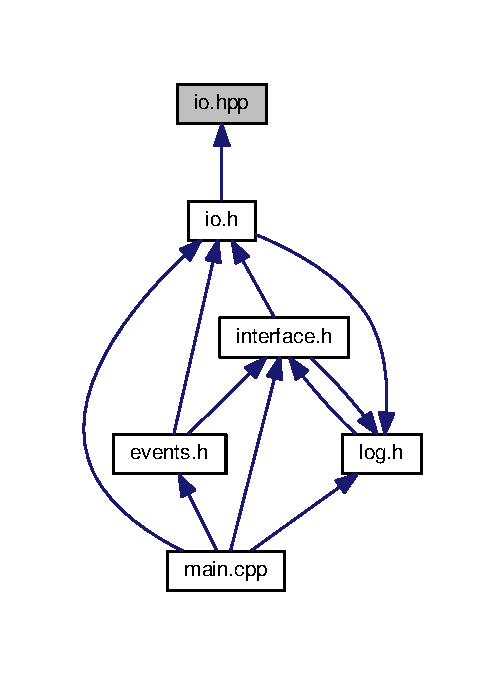
\includegraphics[width=242pt]{io_8hpp__dep__incl}
\end{center}
\end{figure}


\subsection{Detailed Description}
\begin{DoxyAuthor}{Author}
Team 3 
\end{DoxyAuthor}
\begin{DoxyDate}{Date}

\end{DoxyDate}

\hypertarget{log_8hpp}{}\section{log.\+hpp File Reference}
\label{log_8hpp}\index{log.\+hpp@{log.\+hpp}}
This graph shows which files directly or indirectly include this file\+:\nopagebreak
\begin{figure}[H]
\begin{center}
\leavevmode
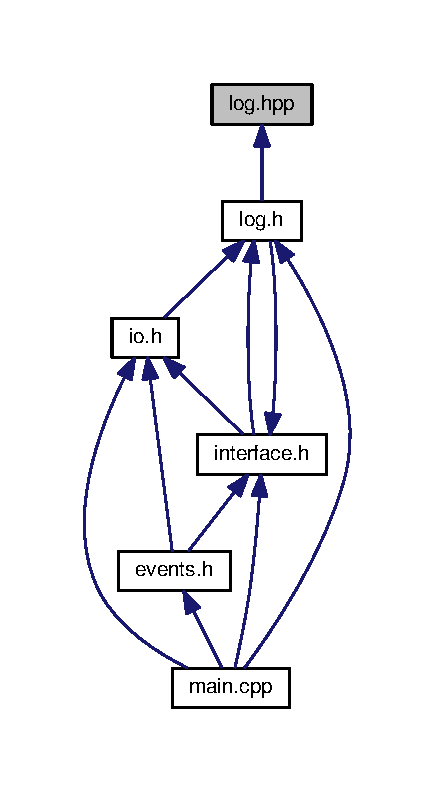
\includegraphics[width=209pt]{log_8hpp__dep__incl}
\end{center}
\end{figure}


\subsection{Detailed Description}
\begin{DoxyAuthor}{Author}
Team 3 
\end{DoxyAuthor}
\begin{DoxyDate}{Date}

\end{DoxyDate}

\hypertarget{main_8cpp}{}\section{main.\+cpp File Reference}
\label{main_8cpp}\index{main.\+cpp@{main.\+cpp}}


driver for project  


{\ttfamily \#include $<$iostream$>$}\\*
{\ttfamily \#include \char`\"{}interface.\+h\char`\"{}}\\*
{\ttfamily \#include \char`\"{}io.\+h\char`\"{}}\\*
{\ttfamily \#include \char`\"{}log.\+h\char`\"{}}\\*
{\ttfamily \#include \char`\"{}events.\+h\char`\"{}}\\*
Include dependency graph for main.\+cpp\+:\nopagebreak
\begin{figure}[H]
\begin{center}
\leavevmode
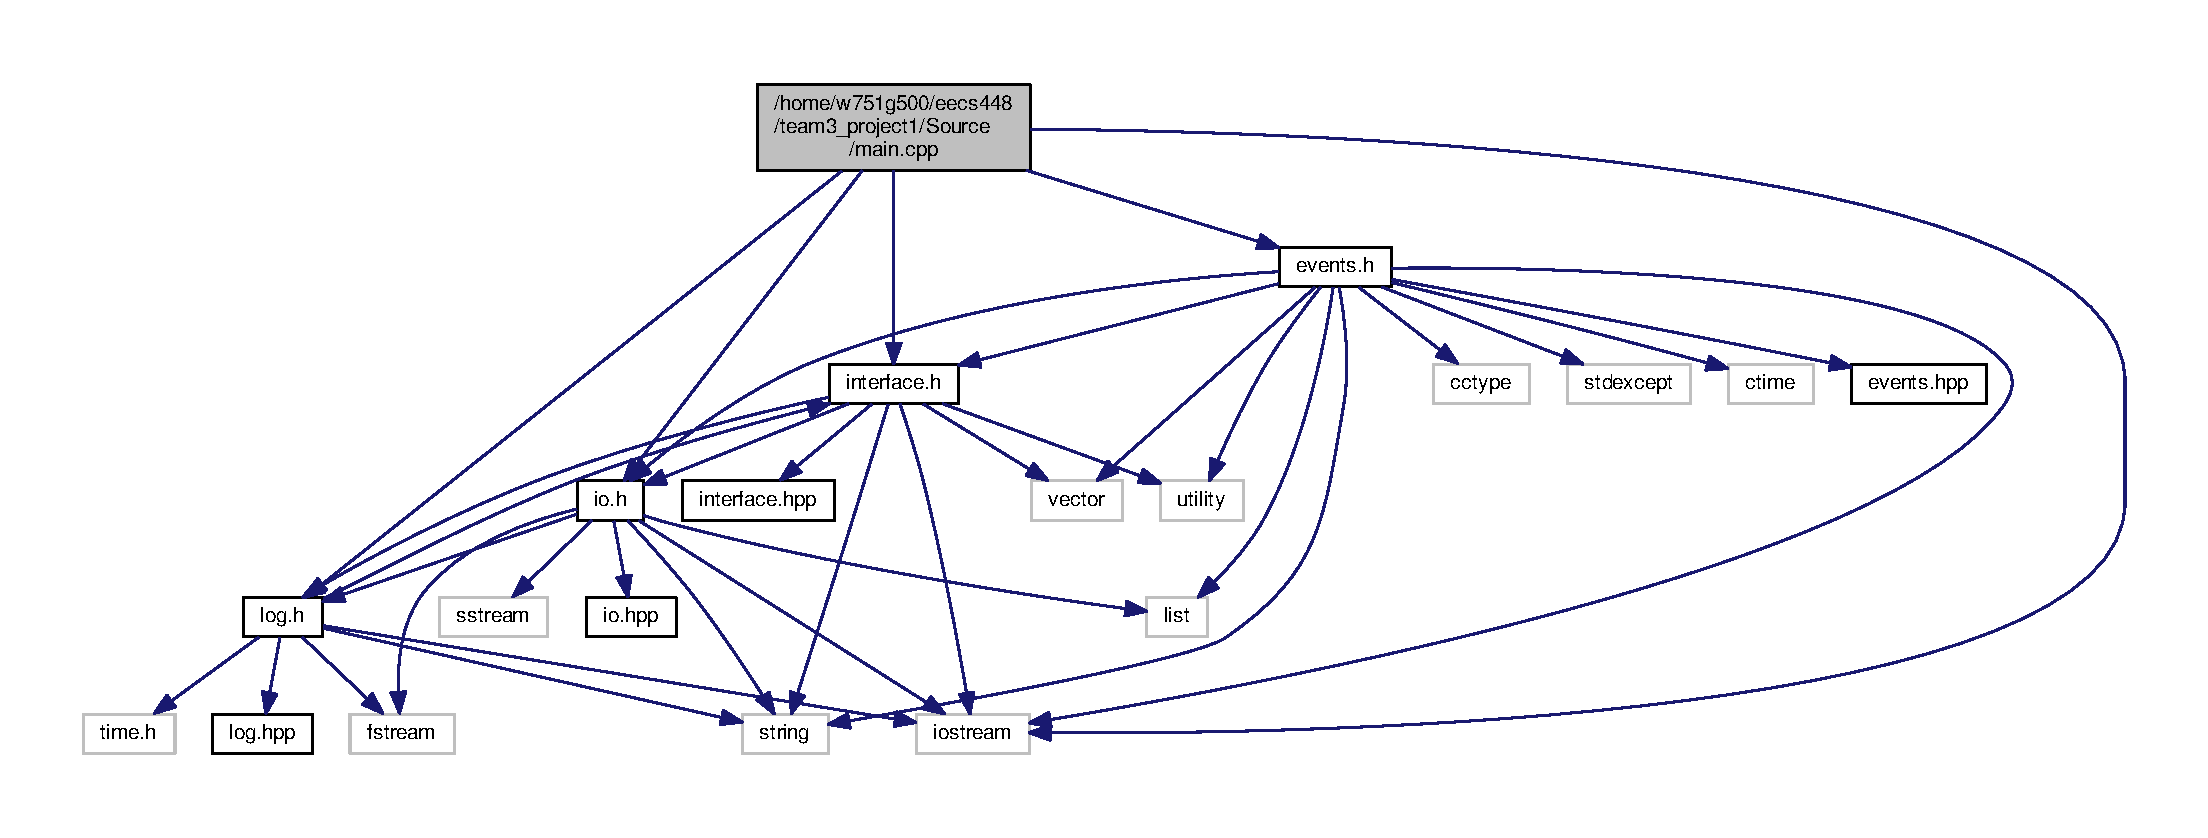
\includegraphics[width=350pt]{main_8cpp__incl}
\end{center}
\end{figure}
\subsection*{Functions}
\begin{DoxyCompactItemize}
\item 
int {\bfseries main} (int argc, char $\ast$$\ast$argv)\hypertarget{main_8cpp_a3c04138a5bfe5d72780bb7e82a18e627}{}\label{main_8cpp_a3c04138a5bfe5d72780bb7e82a18e627}

\end{DoxyCompactItemize}


\subsection{Detailed Description}
driver for project 

\begin{DoxyAuthor}{Author}
Team 3 
\end{DoxyAuthor}
\begin{DoxyDate}{Date}

\end{DoxyDate}

%--- End generated contents ---

% Index
\backmatter
\newpage
\phantomsection
\clearemptydoublepage
\addcontentsline{toc}{chapter}{Index}
\printindex

\end{document}
